\chapter{Développement d'un système de plugins entrées/sorties}

\section{Définition de la mission}
\subsection{Contexte}
Dès le début du développement de Vahana VR, la question des entrées et des sorties
du logicel s'était posée. En effet, Studio étant un logiciel de montage de vidéos
360, ses seules entrées sont des fichiers vidéos, issus des caméras de la monture,
comme présenté dans la section \cf{importation-videos}. De même, la sortie proposée 
est l'équirectangulaire représentant la vidéo 360 obtenue, comme présenté dans la section \cf{exportation}.\\
Ce qui est ici appellé \emph{entrées} sont les données envoyées au programme, quand
les \emph{sorties} sont les données émises par ce programme en retour.\\
Et, contrairement à Studio, pour permettre la vidéo 360 en direct, Vahana VR s'affranchit des fichiers
vidéos importés et propose de capturer directement les images des caméras, via
des cartes d'acquisitions branchées sur la machine utilisée. De même, le logiciel peut émettre 
plusieurs fluxs en sortie permettant, par exemple, le \textit{streaming} ou encore la réémissions vers
une carte d'acquisition, l'export d'un equirectangulaire sous forme de fichier
sur le disque dur étant toujours possible.\\
\begin{figure}
  \centering
  \caption{Schéma des entrées/sorties de Vahana VR}
\end{figure}

\subsection{Problématique}
Dès lors, Vahana VR étant destiné à des sociétés de production, le logiciel doit
être compatible avec un maximum de standards, caméras et cartes d'acquisitions vidéos
pour être facilement adopté. Cependant, tout matériel informatique récquérant des pilotes
\footnote{Programme permettant au système d'exploitation d'interagir avec le matériel couvert par ce pilote\cite{pilote-informatique}.}
, et, les besoins des clients en entrées-sorties n'étant pas les mêmes, il n'était
alors pas possible de concevoir un logiciel monolithique contenant tous les programmes 
d'entrées-sorties supportés~: chaque installation du logiciel aurait requis au client 
une installation de l'ensemble des pilotes.\\
De plus, un client pourrait souhaiter utiliser du matériel entrée/sortie encore
non supporté. Il serait intéressant qu'il puisse réaliser son propre développement
dans l'ecosystème de Vahana VR; ainsi le logiciel pourrait devenir virtuellement
compatible avec n'importe quel standard, caméra ou carte d'acquisition.\\
Il fallait donc développer un système assurant à la fois la compatibilité
entre Vahana VR et ces matériels, et intégrant les contraintes exposées.\\

\subsection{Objectifs}
Au début de ce stage, une solution avait déjà été esquissée et était déjà en partie
mise à l'\oe uvre. Cependant un certain travail était encore nécessaire.\\
L'approche retenue de cette solution est celle de la \emph{Programmation Orientée Composant} (POC),
qui permet une certaine modularité dans l'architecture du projet\cite{poc}. Ainsi chaque nouvelle
carte d'acquisition donnera lieu à un nouveau composant, sous forme d'un \textit{plugin},
qui pourra être distribué, chargé et utilisé si nécessaire\cite{plugin}.\\
\newline
Les objectifs retenus pour cette mission ont donc été~:
\begin{itemize}
  \item Développer les entrées HDMI\footnote{\textit{High Definition Multimedia Interface}, 
  norme de diffusion audio/vidéo numérique\cite{hdmi}.} et SDI\footnote{\textit{Serial Digital Interface}, 
  protocole de diffusion vidéo numérique\cite{sdi}.}.
  \item Développer les sorties HDMI et SDI.
  \item Développer des entrées-sorties Ethernet et PCIe\footnote{\textit{PCI Express}, standard
  de connexion de cartes d'extension sur la carte mère d'un ordinateur\cite{pci-express}.}
  spécifiques, à la demande d'un client.
  \item Déployer l'ensemble des \textit{plugins} sur un dépôt séparé.
  \item Documenter et vérifier la bonne intégration des plugins dans Vahana VR.
\end{itemize}

\begin{figure}
  \centering
  \begin{minipage}{0.2\textwidth}
    \centering
    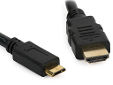
\includegraphics[width=3cm]{images/hdmi-cable.jpg}
    \captionof{subfigure}{HDMI}
  \end{minipage}%
  \hspace{0.03\textwidth}
  \begin{minipage}{0.2\textwidth}
    \centering
    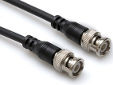
\includegraphics[width=3cm]{images/sdi-cable.jpg}
    \captionof{subfigure}{SDI}
  \end{minipage}%
  \hspace{0.03\textwidth}
  \begin{minipage}{0.2\textwidth}
    \centering
    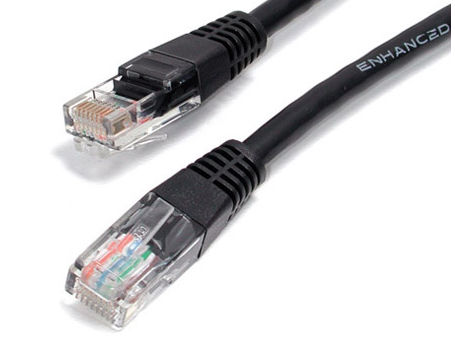
\includegraphics[width=3cm]{images/ethernet-cable.jpg}
    \captionof{subfigure}{Ethernet}
  \end{minipage}%
  \hspace{0.03\textwidth}
  \begin{minipage}{0.2\textwidth}
    \centering
    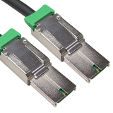
\includegraphics[width=3cm]{images/pcie-cable.jpg}
    \captionof{subfigure}{PCIe}
  \end{minipage}
  \caption{Illustration des différents connecteurs utilisées par Vahana VR}
\end{figure}


\section{Réalisation}
\subsection{Architecture de la solution}
Il s'agissait tout d'abord de saisir le concept de la Programmation Orientée Composant, et la manière
dont il est appliqué pour Vahana VR.\\
Cette approche propose d'utiliser différents \emph{composants}, ou \textit{plugins},
qui vont interragir entre eux~: ici les plugins entrées/sorties avec Vahana VR. On entend
par composant, des bibliothèques (fichiers .dll) qui peuvent être chargées et utilisées
par un programme client, ici Vahana VR. Tout comme les dépendances\footnote{Présentées dans 
la section \cf{integration-dependances-player}.}, un composant va fournir un ensemble
de fonctions, déclarées dans les \textit{headers} qui accompagnent les
fichiers bibliothèques compilés. Ces fonctions sont donc regroupées dans un module externe
au logiciel qui peut y faire appel si besoin, ou non.\\
L'intérêt d'une telle approche est qu'elle permet de développer les plugins séparément du logiciel
logiciel client. Un composant peut également être réutilisé par d'autres programmes~: en ce sens, la POC trouve
des similitudes avec la POO\footnote{Programmation Orientée Objet}.\\
Enfin, si l'analogie avec les dépendances pouvait être faite jusqu'ici, contrairement à ces
dernières dont l'utilisation est réalisée \enquote{en dur} dans le code, un composant
peut être remplacé ou d'autres ajoutés. En effet, le programme recense les composants
présents et tente de les charger \emph{dynamiquement} selon une interface attendue, celle du
\textit{header}~: le code de la bibliothèque est inconnu car compilé, seul sont
connue les fonctions attendues du composant.\\
Un exemple de plugins, est typiquement les extensions d'un navigateur web. Ces composants
ont été écrits pour le navigateur, en répondant à une interface attendue par ce logiciel,
et peuvent être activés ou désactivés à volonté par l'utilisateur.\\
\newline
Ainsi, lors de son exécution, Vahana VR va chercher les bibliothèques présentes dans le dossier
\mintinline{shell-session}{plugins} à sa racine et charge celles présentant ces interfaces.\\
\newline

\subsection{Conception type d'un plugin}
Concrètement, un plugin pour Vahana VR est composé en trois parties~:
\begin{itemize}
  \item Une interface pour créer une entrée.
  \item Une interface pour créer une sortie.
  \item Une interface \textit{discovery} dont le rôle est d'indiquer les possibilités
    de créations entrées/sorties.
\end{itemize}
sdk, driver, programme test

doc, samples

reader

writer

discovery

\subsection{Quelques difficultés et solutions spécifiques}
yuan et wrapper

decklink et design pattern decorator

loadunpacker teledyne

ximea cuda


\section{Déploiement}
\subsection{Création du dépôt VideoStitch-IO}
Les plugins étaient à l'origine développés dans le dépôt VideoStitch-apps. Il faisait
cependant plus sens qu'ils soient déplacés dans un dépôt distinct. Cette opération
nécessitait, comme dans la section \cf{integration-apps}, un déplacement du dossier
de développement et de l'historique des modifications. La technique présentée en annexe~
\ref{deplacer-historique-depots} (p.\pageref{deplacer-historique-depots}) fut de
nouveau utilisée avec succès, déplacant le contenu du dossier \mintinline{shell-session}{src/plugins/}
vers le dossier \mintinline{shell-session}{src/} sur le dépôt VideoStitch-IO.\\
\newline
Ce nouveau dépôt a été organisé de manière sensiblement équivalente à celui de VideoStitch-apps, 
cependant la chaîne de compilation des plugins fut mise à jour pour prendre en compte
cette nouvelle organisation.\\
En outre, ce dépôt nécessitait, tout comme VideoStitch-apps, du VideoStitch-SDK et des dépendances
pour être compilé. Le script \mintinline{shell-session}{update.sh}\footnote{Voir la section \cf{integration-apps}.}
fut alors partagé, et les plugins purent être compilés à nouveau.\\
\newline
Le Buildbot fut alors mis à jour également d'un nouveau builder prenant en charge ce dépôt.
Une liste d'étapes similaires au listing~\ref{windows-apps} (p.\pageref{windows-apps}) furent écrites pour
compiler automatiquement les plugins et les mettre à disposition sur une page de 
téléchargement interne.\\
Enfin, le script \mintinline{shell-session}{update.sh} a été augmenté pour télécharger
la dernière version des plugins et les copier dans la copie du dépôt VideoStitch-apps
du développeur appellant le script. Les plugins ont été déplacés sur un autre dépôt
mais reste toujours nécessaire pour générer l'installateur de Vahana VR et pour
son utilisation.

\subsection{Documentation}
grandes lignes, comment shippé avec plugin et vahana

\subsection{Tests et \textit{QA} de l'intégration des plugins}


\section{Bilan et suite}

